% POWER AGAINST THE NUMBER OF DYADS, from
% scripts/validate_analysis_pipeline.py, 6000 simulated studies per point.
% Three curves because the design carries ONE number and the analysis that
% will be run reports three different things.
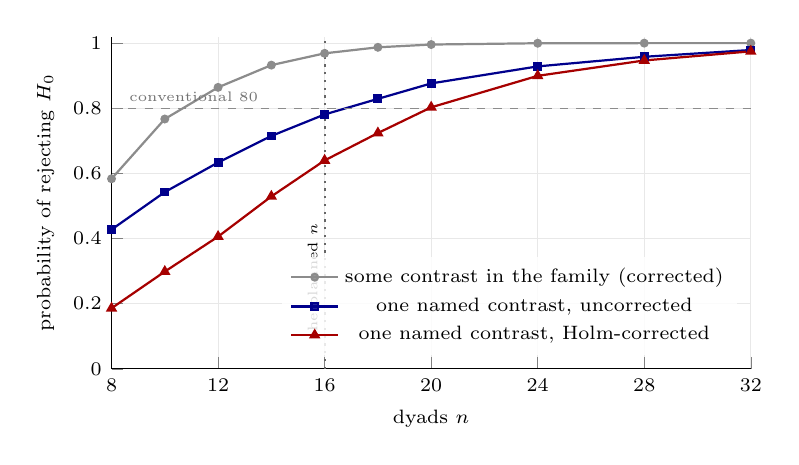
\begin{tikzpicture}
\begin{axis}[
    width=0.80\linewidth, height=58mm,
    xmin=8, xmax=32, ymin=0, ymax=1.02,
    xlabel={dyads $n$}, ylabel={probability of rejecting $H_0$},
    xlabel style={font=\scriptsize}, ylabel style={font=\scriptsize},
    tick label style={font=\scriptsize},
    legend style={font=\scriptsize, at={(0.98,0.04)}, anchor=south east,
                  draw=none, fill=white, fill opacity=0.85, text opacity=1},
    axis lines*=left, grid=major, grid style={gray!18},
    xtick={8,12,16,20,24,28,32},
]
\addplot[black!45, thick, mark=*, mark size=1.2pt] coordinates {
  (8,0.5835) (10,0.7670) (12,0.8642) (14,0.9325) (16,0.9687)
  (18,0.9872) (20,0.9957) (24,0.9997) (28,1.0000) (32,1.0000)};
\addlegendentry{some contrast in the family (corrected)}
\addplot[blue!55!black, thick, mark=square*, mark size=1.2pt] coordinates {
  (8,0.4275) (10,0.5427) (12,0.6335) (14,0.7150) (16,0.7810)
  (18,0.8289) (20,0.8763) (24,0.9286) (28,0.9581) (32,0.9789)};
\addlegendentry{one named contrast, uncorrected}
\addplot[red!65!black, thick, mark=triangle*, mark size=1.6pt] coordinates {
  (8,0.1859) (10,0.2985) (12,0.4059) (14,0.5293) (16,0.6398)
  (18,0.7239) (20,0.8029) (24,0.8996) (28,0.9468) (32,0.9748)};
\addlegendentry{one named contrast, Holm-corrected}
\draw[black!45, dashed] (axis cs:8,0.8) -- (axis cs:32,0.8);
\node[font=\tiny, black!55, anchor=west] at (axis cs:8.3,0.835) {conventional \SI{80}{\percent}};
\draw[black!60, dotted, thick] (axis cs:16,0) -- (axis cs:16,1.02);
\node[font=\tiny, anchor=south west, rotate=90] at (axis cs:16.2,0.06) {the planned $n$};
\end{axis}
\end{tikzpicture}
